\documentclass[journal,12pt,twocolumn]{IEEEtran}

\usepackage{setspace}
\usepackage{gensymb}

\singlespacing


\usepackage[cmex10]{amsmath}

\usepackage{amsthm}

\usepackage{mathrsfs}
\usepackage{txfonts}
\usepackage{stfloats}
\usepackage{bm}
\usepackage{cite}
\usepackage{cases}
\usepackage{subfig}

\usepackage{longtable}
\usepackage{multirow}

\usepackage{enumitem}
\usepackage{mathtools}
\usepackage{steinmetz}
\usepackage{tikz}
\usepackage{circuitikz}
\usepackage{verbatim}
\usepackage{tfrupee}
\usepackage[breaklinks=true]{hyperref}
\usepackage{graphicx}
\usepackage{tkz-euclide}
\usepackage{float}

\usetikzlibrary{calc,math}
\usepackage{listings}
    \usepackage{color}                                            %%
    \usepackage{array}                                            %%
    \usepackage{longtable}                                        %%
    \usepackage{calc}                                             %%
    \usepackage{multirow}                                         %%
    \usepackage{hhline}                                           %%
    \usepackage{ifthen}                                           %%
    \usepackage{lscape}     
\usepackage{multicol}
\usepackage{chngcntr}

\DeclareMathOperator*{\Res}{Res}

\renewcommand\thesection{\arabic{section}}
\renewcommand\thesubsection{\thesection.\arabic{subsection}}
\renewcommand\thesubsubsection{\thesubsection.\arabic{subsubsection}}

\renewcommand\thesectiondis{\arabic{section}}
\renewcommand\thesubsectiondis{\thesectiondis.\arabic{subsection}}
\renewcommand\thesubsubsectiondis{\thesubsectiondis.\arabic{subsubsection}}


\hyphenation{op-tical net-works semi-conduc-tor}
\def\inputGnumericTable{}                                 %%

\lstset{
%language=C,
frame=single, 
breaklines=true,
columns=fullflexible
}
\begin{document}
\newtheorem{theorem}{Theorem}[section]
\newtheorem{problem}{Problem}
\newtheorem{proposition}{Proposition}[section]
\newtheorem{lemma}{Lemma}[section]
\newtheorem{corollary}[theorem]{Corollary}
\newtheorem{example}{Example}[section]
\newtheorem{definition}[problem]{Definition}

\newcommand{\BEQA}{\begin{eqnarray}}
\newcommand{\EEQA}{\end{eqnarray}}
\newcommand{\define}{\stackrel{\triangle}{=}}
\bibliographystyle{IEEEtran}
\providecommand{\mbf}{\mathbf}
\providecommand{\pr}[1]{\ensuremath{\Pr\left(#1\right)}}
\providecommand{\qfunc}[1]{\ensuremath{Q\left(#1\right)}}
\providecommand{\sbrak}[1]{\ensuremath{{}\left[#1\right]}}
\providecommand{\lsbrak}[1]{\ensuremath{{}\left[#1\right.}}
\providecommand{\rsbrak}[1]{\ensuremath{{}\left.#1\right]}}
\providecommand{\brak}[1]{\ensuremath{\left(#1\right)}}
\providecommand{\lbrak}[1]{\ensuremath{\left(#1\right.}}
\providecommand{\rbrak}[1]{\ensuremath{\left.#1\right)}}
\providecommand{\cbrak}[1]{\ensuremath{\left\{#1\right\}}}
\providecommand{\lcbrak}[1]{\ensuremath{\left\{#1\right.}}
\providecommand{\rcbrak}[1]{\ensuremath{\left.#1\right\}}}
\theoremstyle{remark}
\newtheorem{rem}{Remark}
\newcommand{\sgn}{\mathop{\mathrm{sgn}}}
\providecommand{\abs}[1]{\vert#1\vert}
\providecommand{\res}[1]{\Res\displaylimits_{#1}} 
\providecommand{\norm}[1]{\lVert#1\rVert}
%\providecommand{\norm}[1]{\lVert#1\rVert}
\providecommand{\mtx}[1]{\mathbf{#1}}
\providecommand{\mean}[1]{E[ #1 ]}
\providecommand{\fourier}{\overset{\mathcal{F}}{ \rightleftharpoons}}
%\providecommand{\hilbert}{\overset{\mathcal{H}}{ \rightleftharpoons}}
\providecommand{\system}{\overset{\mathcal{H}}{ \longleftrightarrow}}
	%\newcommand{\solution}[2]{\textbf{Solution:}{#1}}
\newcommand{\solution}{\noindent \textbf{Solution: }}
\newcommand{\cosec}{\,\text{cosec}\,}
\providecommand{\dec}[2]{\ensuremath{\overset{#1}{\underset{#2}{\gtrless}}}}
\newcommand{\myvec}[1]{\ensuremath{\begin{pmatrix}#1\end{pmatrix}}}
\newcommand{\mydet}[1]{\ensuremath{\begin{vmatrix}#1\end{vmatrix}}}
\numberwithin{equation}{subsection}
\makeatletter
\@addtoreset{figure}{problem}
\makeatother
\let\StandardTheFigure\thefigure
\let\vec\mathbf
\renewcommand{\thefigure}{\theproblem}
\def\putbox#1#2#3{\makebox[0in][l]{\makebox[#1][l]{}\raisebox{\baselineskip}[0in][0in]{\raisebox{#2}[0in][0in]{#3}}}}
     \def\rightbox#1{\makebox[0in][r]{#1}}
     \def\centbox#1{\makebox[0in]{#1}}
     \def\topbox#1{\raisebox{-\baselineskip}[0in][0in]{#1}}
     \def\midbox#1{\raisebox{-0.5\baselineskip}[0in][0in]{#1}}
\vspace{3cm}
\title{ASSIGNMENT 4}
\author{Vishwanath Hurakadli\\ AI20BTECH11023}
\maketitle
\newpage
\bigskip
\renewcommand{\thefigure}{\theenumi}
\renewcommand{\thetable}{\theenumi}
Download all python codes from
\begin{lstlisting}
https://github.com/vishwahurakadli/EE3900/blob/main/Assignment_4/EE3900_Assignment_4.ipynb
\end{lstlisting} 
and latex-tikz codes from 
\begin{lstlisting}
https://github.com/vishwahurakadli/EE3900/blob/main/Assignment_4/EE3900_Assignment_4.tex
\end{lstlisting}
%
\section{Problem}
(Linear Forms-2.27)\\
Find the equation of the plane passing through the intersection of the planes $\myvec{2&2&-3}\vec{x} = 7$ and $\myvec{2&5&3}\vec{x} = 9$ and the point $\myvec{2\\1\\3}$
\section{Solution}
General equation of plane is given by
\begin{align}
    \vec{n}^T\vec{x} = c
\end{align}
The equation of a plane $P$ passing through the intersection of two planes $P_{1}$ and $P_{2}$ is given by,
\begin{align}
   P : P_{1} + \lambda P_{2}\label{eq1}
\end{align}
\begin{lemma}
The equation of a plane passing through the intersection of two planes and given point will be\\
\begin{align}
P : P_{1} + \lambda P_{2}\label{eq1}
\end{align}
Let planes $P_{1}$ and $P_{2}$ respectively given by
\begin{align}
\vec{n_{1}}^T\vec{x}&=c_{1}\\ \vec{n_{2}}^T\vec{x}&=c_{2}
\end{align}
Plane $P$  is given by 
\begin{align}
\vec{n^T\vec{x}}&=c
\end{align}
Point through which Plane $P$ is passing is $A$\\
where
\begin{align}
\vec{n}^T &= \vec{n_{1}}^T + \brak{\frac{c_{1} - \vec{n_{1}}^T\vec{A}}{\vec{n_{2}}^T\vec{A}- c_{2}}}\vec{n_{2}}^T\\
c &= c_{1} + \brak{\frac{c_{1} - \vec{A}\vec{n_{1}}^T}{\vec{A}\vec{n_{2}}^T- c_{2}}}c_{2}
\end{align}
\end{lemma}
\begin{proof}
Plane $P$ passing through the intersection of two planes will be
\begin{align}
\vec{n_{1}}^T\vec{x} + \lambda\brak{\vec{n_{2}}^T\vec{x}} = c_{1} + \lambda\brak{c_{2}}\\
\implies \brak{\vec{n_{1}}+\lambda\vec{n_{2}}}^T\vec{x} = c_{1} + \lambda\brak{c_{2}}
\end{align}
Then
\begin{align}\label{eq:12}
\vec{n}^T &= \vec{n_{1}}^T + \lambda\vec{n_{2}}^T\\
c &= c_{1} + \lambda c_{2}
\end{align}
Given that plane $P$ passes through point $\vec{A}$ then
\begin{align}
\brak{\vec{n_{1}}+\lambda\vec{n_{2}}}^T\vec{A} &= c_{1} + \lambda\brak{c_{2}}\\
\implies \lambda &= \frac{c_{1} - \vec{n_{1}}^T\vec{A}}{\vec{n_{2}}^T\vec{A}- c_{2}}
\end{align}
Substituting $\lambda$ in \eqref{eq:12}
\begin{align}
\vec{n}^T &= \vec{n_{1}}^T + \brak{\frac{c_{1} - \vec{n_{1}}^T\vec{A}}{\vec{n_{2}}^T\vec{A}- c_{2}}}\vec{n_{2}}^T\\
c &= c_{1} + \brak{\frac{c_{1} - \vec{n_{1}}^T\vec{A}}{\vec{n_{2}}^T\vec{A}- c_{2}}}c_{2}
\end{align}
\end{proof}
For the given problem 
\begin{align}
\vec{n_{1}}=\myvec{2\\2\\-3}\\
\vec{n_{2}} =\myvec{2\\5\\3}\\
c_{1} = 7\\
c_{2} = 9
\end{align}
By solving the given values
\begin{align}
\lambda &= \frac{10}{9}\\
\vec{n} &= \myvec{\frac{38}{9}\\\frac{68}{9}\\\frac{1}{3}}\\
c &= 17
\end{align}
So the equation of plane $P$ is given by
\begin{align}
\myvec{\frac{38}{9}&\frac{68}{9}&\frac{1}{3}}\vec{x} &= 17
\end{align}
\begin{figure}[!ht]
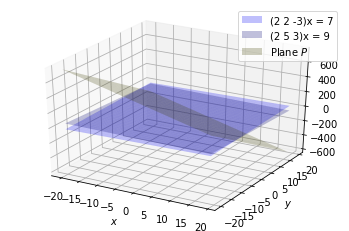
\includegraphics[ width=\columnwidth]{EE3900_Assignment_4.png}
\caption{Plane $P$ passing through intersection of $P_{1}$ and $P_{2}$ and through a point $\vec{A}$}
\label{fig:Line }	
\end{figure}
\end{document}
\end{document}
